\documentclass[12pt]{article}
\usepackage[margin=1in]{geometry}
\usepackage[all]{xy}
\usepackage{tikz}


\usepackage{amsmath,amsthm,amssymb,color,latexsym}
\usepackage{geometry}        
\geometry{letterpaper}    
\usepackage{graphicx}

\newtheorem{problem}{Problem}

\newenvironment{solution}[1][\it{Solution}]{\textbf{#1. } }{$\square$}

\newcommand*\mycirc[1]{%
  \begin{tikzpicture}
    \node[draw,circle,inner sep=1pt] {#1};
  \end{tikzpicture}}
  
\begin{document}
\noindent E0 225 Design \& Analysis of Algorithms\hfill \textbf{Assignment - 2}\\
Sai Phanindra Korlepara | \textbf{24142} | M.Tech CSA Dept.

\hrulefill %%%%%%%%%%%%%%%%%%%%%%%%%%%%%%%%%%%%%%%%%%%%%%%%%%%%%%%%%%%%%%%%%%%%%%%%%%%%%%%%%%%%%%%%%%%%
\\
\begin{problem}
 JE Book, Chapter 3, Problem 1C. \\
 \indent In a previous life, you worked as a cashier in the lost Antarctican colony of Nadiria, spending the better part of your day giving change to your customers. Because paper is a very rare and valuable resource in Antarctica, cashiers were required by law to use the fewest bills possible whenever they gave change. Thanks to the numerological predilections of one of its founders, the currency of Nadiria, called Dream-Dollars, was available in the following denominations: \$1, \$4, \$7, \$13, \$28, \$52, \$91, and \$365.\\
 \indent (c) Describe a dynamic programming algorithm that computes, given an integer k, the minimum number of bills needed to make k Dream-Dollars.
\end{problem}

%%%%%%%%%%%%%%%%%%%%%%%%%%%%%%%%%%%%%%%%%%%%%%%%%%%%%%%%%%%%%%%%%%%%%%%%%%%%%%%%%%%%%%%%%%%%%%%%%%%%%%%

\begin{solution}
	A greedy algorithm doesn't give optimal solution to this problem for all the numbers. For example if the integer $k$ was 416, the greedy algorithm would output $7 (365 - 28 - 13 - 7 - 1 - 1 -1)$, but the real optimal solution is $5 (91 - 91 - 91 -91 - 52)$. 
 \\ \indent Instead we can formulate a dynamic algorithm that takes advantage of the optimal sub-structure property of this algorithm. Any optimal solution would be of the format, 
 
 \begin{equation*}
        Target = Best(Value_{Possible \space Denomination} + Solution(Target - Value)     
 \end{equation*}
  
 \\ \\\textbf{Algorithm} \\
\begin{enumerate}
    \item In this bottom-up Dynamic algorithm, we loop from $i = 1$ to $i= k$, where $k$ is the target value. 
    \item  In any given iteration, $i$, the optimum solutions for all the possible values less than $i$, are already estimated. 
    \item To find the optimal solution for the value $i$ , we will loop once for each of the possible denominations. 
    \item  If the current denomination under consideration is $d$, then any possible optimal solution for the value $i$ that uses $d$ would need $1+solution(i-d)$ notes. Here $1$ is for the denomination under current consideration.
    \item The $min(1+solution(i-d))$ is considered the optimal solution for $i$. 
    \item We keep doing iterations for higher $i$s, till the $k$th iteration is finished, which will give the minimal number of notes needed to reach the target value $k$.  \\
\end{enumerate}
\textbf{\indent Runtime Analysis} \\  
\indent User calls denomCounter function.  Two loops nested in one another. One that runs $k$ times, the other runs $d$ times.  The runtime analysis for this algorithm is simply $O(dk)$.\\ \\
\indent 
\\
\textbf{Sample C Code} 
\begin{verbatim}
// user calls denomCounter 
int denomCounter (int *denoms, int size, int target){
    int result, * interimResult = (int *) malloc ((target+1) * sizeof(int));
    
    for (int i = 0; i <= target; i++){
        int k = 0;
        interimResult[i] = i;
        
        while(*(denoms+k) <= i && k < size){
            if(interimResult[i] > 1+interimResult[i-*(denoms+k)])
                interimResult[i] = 1+interimResult[i-*(denoms+k)];
            k++;
        }
    }
    
    result = interimResult[target];
    free(interimResult);
    return result;
}
\end{verbatim}

\textbf{Proof of Correctness}\\ 
\indent Claim : The problem of choosing minimum number of bills possible to reach a target value has optimal sub structure property. 
\begin{itemize}
    \item  Let's prove the property using Proof by Induction. 
    \item \textbf{Base case : } In all the cases where $target$ is equal to one of the denominations $denoms[i]$, The algorithm always chooses 1. 
    \begin{itemize}
        \item To prove this, we can see that in the inner while loop, we check once for each compatible denomination, we choose the best of $(1+interimResult[i-*(denoms+k)])$. 
        \item For the case where $*(denoms+k) = target$ ie, where $i=target$, $(1+interimResult[i-*(denoms+k)])$ will equate to $1+interimResult[0]$, which would be $1$. 
        \item In any of the other cases, $(1+interimResult[i-*(denoms+k)])$ will at best equate to 2 as $i-*(denoms+k) \neq 0$. 
        \item Hence in the base case, where target is one of the denominations the algorithm always chooses 1.
    \end{itemize}
    \item \textbf{Inductive Step : } If we assume that all the results till $interimResult[i-1]$ is optimal, Prove that the $i$th step will also be optimal
    \begin{itemize}
        \item Any optimal solution to minimize the number of bills required to reach a target value will only use bills of the denominations that are available. 
        \item For any non zero target value, any optimal solution must use atleast one of all the possible denominations. 
        \item Since the inner while loops checks once with each possible denomination and since all of the $interimResult[1]$ to $interimResult[i-1]$ is optimal as per the assumption, $interimResult[i-*(denoms+k)]$ chosen during any of the iterations of while loop is also optimal. 
        \item Hence the optimal solution for the target value would be considered in one of the loop iterations. 
    \end{itemize}
    \item By proving Base case and Inductive step, We have proved that the algorithm will give optimal solution using Proof by Induction. 
\end{itemize}
Note : An assumption made with this algorithm is that all the requests for target value is integers \& that any positive integer can be enumerated from the given denominations. 
\end{solution} 

\hrulefill %%%%%%%%%%%%%%%%%%%%%%%%%%%%%%%%%%%%%%%%%%%%%%%%%%%%%%%%%%%%%%%%%%%%%%%%%%%%%%%%%%%%%%%%%%%%

\begin{problem}
 JE Book, Chapter 3, Problem 3B. \\
 \indent Suppose you are given an array $A[1 .. n]$ of numbers, which may be positive, negative, or zero, and which are not necessarily integers.
\\ \indent (b) Describe and analyze an algorithm that finds the largest product of
elements in a contiguous subarray $A[i .. j]$.
\\ \indent  Given the one-element array $[-374]$ as input, your second algorithm should return $1$. (The empty interval is still an interval!) For the sake of analysis, assume that comparing, adding, or multiplying any pair of numbers takes O(1) time.
\end{problem}

%%%%%%%%%%%%%%%%%%%%%%%%%%%%%%%%%%%%%%%%%%%%%%%%%%%%%%%%%%%%%%%%%%%%%%%%%%%%%%%%%%%%%%%%%%%%%%%%%%%%%%%

\begin{solution}
	This problem deals with many edge cases and needs to be handled carefully. As per the note given under the problem, We also have to consider the empty interval for any given array. So the highest product will always have to be $> =1$.   \\
 \indent The main motivation to this algorithm is as follows, we will calculate the cumulative product from the start to the end of the array. First let's assume that the numbers in the input array are always positive ie, $\geq 0$. We will handle the cases with negative elements later. \\
 \indent We start from the begining to the end of the array, calculating cumulative at each stage. Since all the elements are positive, the value of cumulative always stays $\geq 0$. Since the input array contains real numbers it is possible we might encounter elements such as $0$ or $0.00001$ (an arbitrarily small number). \\
 \indent If suppose the cumulative estimated till $i$th element is say $c \mid c \geq 1$. After encountering such a small element if the cumulative product comes down to a value $<1$ ie, $c*arr[i] < 1$, any possible $maxProduct$ will not contain this $i$th element. If $d$ is the best possible max product that starts at $i+1$th element we can see the following
\begin{gather*}
    c \geq 1 > c \cdot \text{arr}[i] \geq 0 \\
    \max(c,d) > \text{arr}[i] \cdot d > c \cdot \text{arr}[i] \cdot d > c \cdot \text{arr}[i] > \text{arr}[i]
\end{gather*}
because of this reason if the cumulative ever gets down to a value between $0$ \& $1$, we will reset the cumulative to 1, while maintaining the best $maxProduct$ we have encountered yet. \\
\indent Now to consider the cases where there might be negative elements in the array. We will consider the following 2 scenarios. If suppose $i$ \& $j$ are the starting and ending elements of the $maxProduct$ for a given array. 
\\ \indent Case 1 : There are even number of negative numbers in front of the $i$th element. In this case the algorithm discussed above for just positive numbers, will work here as well as by the time we reach $j$th element calculating the cumulative product, it will be positive and recorded as the $best$ that was encountered yet. 
\\ \indent Case 2: There are odd number of negative numbers in front of the $i$th element. In this case the cumulative that is calculated at the $j$th element will be negative and hence it will not be recorded as $best$. 
\\\indent To deal with this case, as we are passing through each element calculating the cumulative product, we will process all the times when cumulative was negative separately. If there are odd number of negative numbers before $i$th element and since $maxProduct$ has to be positive, $j$th element will be negative aswell. 
\\ \indent Each time we encounter a negative cumulative product, we will divide it by the previously encountered negative cumulative product, This number encapsulates the positive contribution of all the elements between this and previous element that has a negative cumulative product. 
\\ \indent We need to do this as because, it is possible that there are even number of negative numbers whose product is positive between current and previous element with negative cumulative product.
\\ \indent The best observed in either of the both possible cases will be taken as the $maxProdcut$ of the given array.  
\\  \textbf{Algorithm} 
\begin{enumerate}
    \item Loop through the array, calculating cumulative product at each element. 
    \item If the calculated product at the current step is between $0$ \& $1$, reset the cumulative product to $1$.
    \item Check if the cumulative product in the current step is greater than the best product yet and update best variable accordingly.
    \item  If the cumulative product is negative, divide it by the most recent previous negative cumulative product. 
    \item Check if this value is compatible with negative cumulative product similar to positive cumulative product and update $negprod$ accordingly. 
    \item Compare the negative side cumulative product with best product and update best accordingly. 
    \item Loop through the array till the entire array is scanned and return the $best$ variable. 
\end{enumerate} 
\textbf{Runtime Analysis} \\
\indent There is one loop running for the length of the array, the runtime complexity is $O(n)$. \\ \\
 \textbf{Sample C Code}
\begin{verbatim}
// user calls maxProduct. calculate is internal function.
// github.com/Phani777/E0-225-DAA-24 for executable.
void calculate (float * maxProd, float * prod , float testProd){
    *prod = (testProd > 1.0 || testProd < 0.0) ? testProd : 1.0;
    *maxProd = (*maxProd > *prod) ? *maxProd : *prod;
}
float maxProduct(float * arr, int size){
    float maxProd = 1.0, posProd = 1.0 , negProd = 1.0, prevProd;
    int negCount=0;

   for(int i = 0; i < size; i++){
        calculate (&maxProd , &posProd , posProd*arr[i]);
        
        if(posProd < 0){
            if (negCount > 0)
                calculate (&maxProd , &negProd , negProd*posProd/prevProd);
             prevProd = posProd; negCount++;
        }
    }
    return maxProd;
}
\end{verbatim}

\end{solution} 

\hrulefill %%%%%%%%%%%%%%%%%%%%%%%%%%%%%%%%%%%%%%%%%%%%%%%%%%%%%%%%%%%%%%%%%%%%%%%%%%%%%%%%%%%%%%%%%%%%

\begin{problem}
 JE Book, Chapter 8, Problem 14. \\
 \indent You just discovered your best friend from elementary school on Twitbook.You both want to meet as soon as possible, but you live in two different cites that are far apart. To minimize travel time, you agree to meet at an intermediate city, and then you simultaneously hop in your cars and start driving toward each other. But where exactly should you meet?
\\ \indent You are given a weighted graph $G = (V, E)$, where the vertices $V$ represent cities and the edges $E$ represent roads that directly connect cities. Each edge $e$ has a weight $w(e)$ equal to the time required to travel between the two cities. You are also given a vertex $p$, representing your starting location, and a vertex $q$, representing your friend’s starting location.
\\ \indent Describe and analyze an algorithm to find the target vertex $t$ that allows
you and your friend to meet as quickly as possible.
\end{problem}

%%%%%%%%%%%%%%%%%%%%%%%%%%%%%%%%%%%%%%%%%%%%%%%%%%%%%%%%%%%%%%%%%%%%%%%%%%%%%%%%%%%%%%%%%%%%%%%%%%%%%%%

\begin{solution}
 The "shortest path" between both the friends' starting points may not contain the city that avails shortest meeting time. Consider a graph with 4 edges, $p,q,r,s$. Where $p$ and $q$ are starting points for the friends and $r,s$ are two potential meeting points. 


\begin{center}
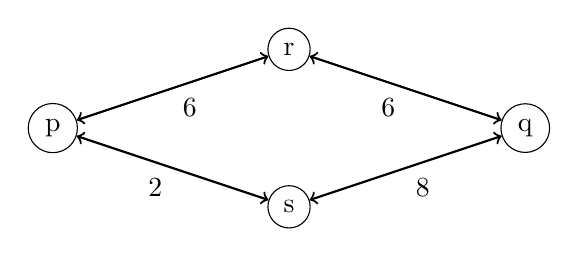
\begin{tikzpicture}[scale=2,auto,swap]
    % Nodes
    \node (p) at (0,0) [circle,draw] {p};
    \node (q) at (3,0) [circle,draw] {q};
    \node (r) at (1.5,0.5) [circle,draw] {r};
    \node (s) at (1.5,-0.5) [circle,draw] {s};

    % Edges with weights
    \path[<->,thick ] (p) edge node {6} (r);
    \path[<->,thick ] (r) edge node {6} (q);
    \path[<->,thick ] (p) edge node {2} (s);
    \path[<->,thick ] (s) edge node {8} (q);
\end{tikzpicture}
\end{center}

\indent The shortest path from $p$ to $q$ would be via $s$, which takes 10 hours. The time taken to meet at the city $s$ would be 8 hours. But the fastest city for both friends to meet would be at the city $r$, where the time taken would be 6 hours. 
\\ \indent But the travel time between the two cities $p$ \& $q$ via $r$ would be 12 hours which is not the shortest path.   To find the shortest time to meet between two cities we can perform dijkstra's algorithm on both the starting points individually.  
\\ \indent Then we can check in linear time to all possible cities for the travel time taken, to assess which city is fastest for both of them to meet. We can use Dijkstra's algorithm because all the edge weights are positive as travel time cannot be negative. \\
\\ \textbf{Algorithm}
\begin{enumerate}
    \item Perform Dijkstra's algorithm with city $p$ as starting point. Save the array of shortest travel time to all the cities in the graph starting from city $p$. 
    \item Perform Dijkstra's algorithm with city $q$ as starting point. Save the array of shortest travel time to all the cities in the graph starting from city $q$. 
    \item In linear time we can consider each one of the cities as possible meeting point, if we are checking  $i$th city as the meeting point. then the travel time to meet at that city would be $max(p[i],q[i])$. 
    \item Whichever city has the smallest travel time is chosen as the meeting point.
\end{enumerate}
\textbf{Runtime Analysis}\\
\indent We are performing Dijkstra's algorithm twice, since the runtime complexity of dijkstra's is $O(v^2)$ , where $v$ is the number of vertices in the graph. The runtime complexity of the first two step is $2O(v^2)$. 
\\ \indent Then we are checking each vertex (city) once for compatibility. The runtime complexity to perform this step is $O(v)$. 
\ \\\indent The total runtime complexity of this algorithm is $2O(v^2)+O(v)$, which equates to $O(v^2)$ overall. 
\end{solution} 

\hrulefill %%%%%%%%%%%%%%%%%%%%%%%%%%%%%%%%%%%%%%%%%%%%%%%%%%%%%%%%%%%%%%%%%%%%%%%%%%%%%%%%%%%%%%%%%%%%

\begin{problem}
 JE Book, Chapter 8, Problem 16. \\
 \indent You are given a directed graph $G = (V, E)$ with non-negatively weighted edges and two vertices $s$ and $t$. Describe and analyze an algorithm to find the shortest walk in $G$ from $s$ to $t$ (possibly repeating vertices and/or edges) whose number of edges is divisible by $3$.

\begin{center}
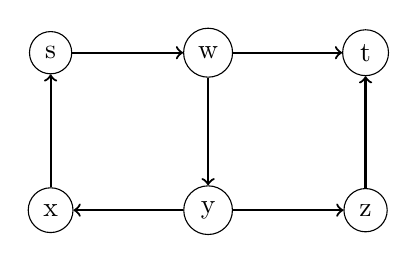
\begin{tikzpicture}[scale=2,auto,swap]
    % Nodes
    \node (s) at (0,0.5) [circle,draw] {s};
    \node (w) at (1,0.5) [circle,draw] {w};
    \node (t) at (2,0.5) [circle,draw] {t};
    \node (x) at (0,-0.5) [circle,draw] {x};
    \node (y) at (1,-0.5) [circle,draw] {y};
    \node (z) at (2,-0.5) [circle,draw] {z};
    % Edges with weights
    \path[->,thick ] (s) edge node {} (w);
    \path[->,thick ] (w) edge node {} (t);
    \path[->,thick ] (x) edge node {} (s);
    \path[->,thick ] (y) edge node {} (x);
    \path[->,thick ] (y) edge node {} (z);
    \path[->,thick ] (z) edge node {} (t);
    \path[->,thick ] (w) edge node {} (y);
\end{tikzpicture}
\end{center}


\indent For example, given the graph shown above, with the indicated vertices $s$
and $t$, and with all edges having weight $1$, your algorithm should return $6$,
which is the length of the walk $s \rightarrow w \rightarrow y \rightarrow x \rightarrow s \rightarrow w \rightarrow t$ has length $6$.
\end{problem}

%%%%%%%%%%%%%%%%%%%%%%%%%%%%%%%%%%%%%%%%%%%%%%%%%%%%%%%%%%%%%%%%%%%%%%%%%%%%%%%%%%%%%%%%%%%%%%%%%%%%%%%

\begin{solution}
	We can use dijkstra's algorithm on a modified graph with separated states for each vertex adding new edges. 
 \\ \textbf{Algorithm}\\
 \begin{enumerate}
     \item For each vertex $v_i$ in the graph insert 3 new vertices, $v_{i,0}$ \& $v_{i,1}$ \& $v_{i,2}$. Each of these 3 new states represent the $mod(walkLength,3)$ taken to reach the vertex $v_i$. 
     \item For each edge $e_k$ in the graph between $v_i$ \& $v_j$ , insert 3 new edges with the same weight $w$ as original edge as follows,  $e_{k,1}$ betwen $v_{i,0}$ \&  $v_{j,(0+w)\%3}$, $e_{k,2}$ betwen $v_{i,1}$ \&  $v_{j,(1+w)\%3}$, $e_{k,3}$ betwen $v_{i,2}$ \&  $v_{j,(2+w)\%3}$.
     \item In the new graph, we want to find the shortest path from $p_{0}$ (instance of starting point with reminder $0$) to $q_{0}$, the source and destinations of the original graph. 
     \item The aim is to make sure that we start with vertex having remainder $0$ and end with vertex having reminder $0$. 
     \item Call Dijkstra's algorithm with $s_{0}$ , $t_{0}$ as arguments as all edges have positive weight. 
     \item The result for this graph is same as walk length of the original graph.
 \end{enumerate}
 \\ \textbf{Runtime Analysis} \\
 \begin{itemize}
     \item In the first step we scanned through each vertex once created $3V$ verticies in total. Total runtime for this step is $O(3V)$. 
     \item In the second step we scanned through each edge once created $3E$ Edges in total. Total runtime for this step is $O(3E)$.
     \item Worst case runtime of Dijkstra algorithm for the given case is $O((3V)^2)$
     \item The total runtime for this algorithm is $O(3V)+O(3E)+O(9V^2)$. Since in the worst case $E = O(V^2)$. The overall worst case runtime complexity for this algorithm is $O(V^2)$
 \end{itemize}
\end{solution} 

\hrulefill %%%%%%%%%%%%%%%%%%%%%%%%%%%%%%%%%%%%%%%%%%%%%%%%%%%%%%%%%%%%%%%%%%%%%%%%%%%%%%%%%%%%%%%%%%%%

\begin{problem}
 JE Book, Chapter 9, Problem 6B. \\
 \indent In this problem we will discover how you, yes you, can be employed by Wall Street and cause a major economic collapse! The arbitrage business is a money-making scheme that takes advantage of differences in currency exchange. In particular, suppose $1$ US dollar buys $120$ Japanese yen, $1$ yen buys $0.01$ euros, and $1$ euro buys $1.2$ US dollars. Then, a trader starting with \$$1$ can convert their money from dollars to yen, then from yen to euros, and finally from euros back to dollars, ending with \$$1.44!$ The cycle of currencies \$ → ¥ → € → \$ is called an arbitrage cycle. Of course, finding and exploiting arbitrage cycles before the prices are corrected requires extremely fast algorithms.
\\ \indent Suppose n different currencies are traded in your currency market. You are given the matrix $Exch[1 .. n, 1 .. n]$ of exchange rates between every pair of currencies; for each $i$ and $j$, one unit of currency $i$ can be traded for $Exch[i, j]$ units of currency $j$. (Do not assume that $Exch[i, j] * Exch[ j, i] = 1$.)
\\ \indent (b) Describe an algorithm to determine whether the given matrix of currency exchange rates creates an arbitrage cycle.
\end{problem}

%%%%%%%%%%%%%%%%%%%%%%%%%%%%%%%%%%%%%%%%%%%%%%%%%%%%%%%%%%%%%%%%%%%%%%%%%%%%%%%%%%%%%%%%%%%%%%%%%%%%%%%

\begin{solution}
	We can take advantage of Bellman Ford algorithm to simplify this problem. If suppose we consider, that each currency is a vertex, and there are two edges connecting any pair of two vertices. If we assume that $-log(Exch[i,j])$ is the weight of the edge going from vertex / currency $i$ to vertex / currency $j$, the sum of the two adjacent edges will be the logarithm of product of the exchange rates.
 \\ \indent We can apply Bellman ford algorithm on this graph to find negative weight cycles. Since Bellman ford runs in $O(VE)$ time. For our current graph $E = O(V^2)$. This means that we can find the presence of a arbitrage cycle in $O(N^3)$ time. 
 \\ \\ \textbf{Algorithm} \\
 \begin{enumerate}
     \item Update each element $E_{i,j}$ in the exchange matrix with $-log(E_{i,j})$. 
     \item Call Bellman-Ford algorithm, with edge weights as the updated Exchange matrix. 
     \item Check for negative weight cycle by performing one more iteration
     \item If the Bellman-Ford algorithm returns True for presence of negative weight cycle, then there is a valid arbitrage cycle in the given exchange matrix. 
 \end{enumerate}
 \\ \textbf{Runtime Analysis} \\ 
 \indent The first step in the algorithm of updating the edge weights takes $O(N^2)$ runtime as there are $N^2$ edges. The bellman ford algorithm takes $O(VE)$ time for a graph with $V$ verticies and $E$ edges.Checking for Negative weight cycle takes another $O(N^2)$ time as there are $N^2$ edges. Since our current graph has $V^2$ edges, the total runtime complexity of this algorithm is $O(V^2)+O(V^2*V)+O(V^2) = O(V^3)$ time.  
\end{solution} 

\hrulefill %%%%%%%%%%%%%%%%%%%%%%%%%%%%%%%%%%%%%%%%%%%%%%%%%%%%%%%%%%%%%%%%%%%%%%%%%%%%%%%%%%%%%%%%%%%%


\end{document}
